\documentclass[25pt, a0paper, portrait]{tikzposter}
\usepackage[T1]{fontenc}
\renewcommand*\familydefault{\sfdefault}
\usepackage{sfmath}
\usepackage{amsmath}
\usepackage{lipsum}
\usepackage[compress]{cite}
\usepackage{graphicx}
\usepackage{siunitx}

\newcommand{\CORE}{The CORE collaboration}
\newcommand{\PLANCK}{The Planck collaboration}
\newcommand{\prd}{PRD}
\newcommand{\prr}{PRR}
\newcommand{\mnras}{MNRAS}
\newcommand{\jcap}{JCAP}
\newcommand{\jmap}{JMAP}
\newcommand{\joss}{JOSS}
\newcommand{\pasa}{PASA}
\newcommand{\aap}{A\&A}
\newcommand{\prl}{PRL}
\newcommand{\arxiv}{arXiv}
\newcommand{\polychord}{\texttt{PolyChord}}

\DeclareSIUnit \parsec {pc}


\makeatletter
\renewcommand\TP@maketitle{%
    \centering
    \vspace{-40pt}
    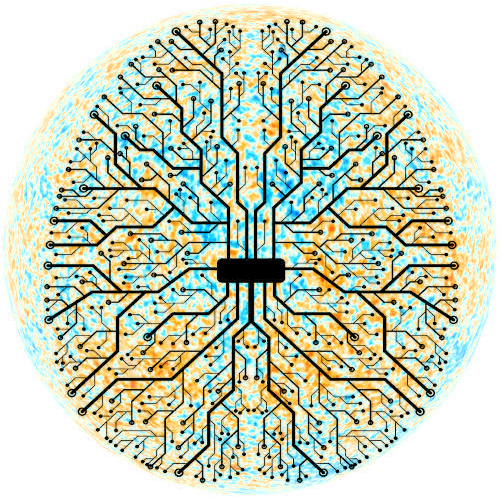
\includegraphics[height=0.11\textwidth]{images/handley-lab.png}\hfill
    \begin{minipage}[b]{0.7\linewidth}
        \centering
        \color{titlefgcolor}
        {\Huge \sc \@title \par}
        \vspace*{1em}
        {\huge \@author \par}
        \vspace*{1em}
        {\LARGE \@institute}
    \end{minipage}%
    \hfill
\includegraphics[height=0.11\textwidth]{images/cambridge-cropped.pdf}
}
\makeatother

\title{Clustering Considerations for Nested Sampling}
\author{Adam Ormondroyd \href{mailto:ano23@cam.ac.uk}{ano23@cam.ac.uk}}
\institute{Kavli Institute for Cosmology $\cdot$ Cavendish Laboratory $\cdot$  University of Cambridge}
%\usetheme{Default}
%\usetheme{Rays}
%\usetheme{Basic}
%\usetheme{Simple}
\usetheme{Envelope}
%\usetheme{Wave}
%\usetheme{Board}
%\usetheme{Autumn}
%\usetheme{Desert}

\tikzposterlatexaffectionproofoff{}

\let\oldbibliography\thebibliography
\renewcommand{\thebibliography}[1]{\oldbibliography{#1}
\setlength{\itemsep}{-5pt}} %Reducing spacing in the bibliography.

\pdfinclusioncopyfonts=1 % Fix fonts on non-linux machines

\usepackage{xcolor}
\definecolor{C0}{HTML}{E06C75}
\definecolor{C1}{HTML}{56B6C2}
\definecolor{C2}{HTML}{56B6C2}
\definecolor{C3}{HTML}{98C07B}
\definecolor{C4}{HTML}{9467bd}
\definecolor{C5}{HTML}{8c564b}
\definecolor{C6}{HTML}{e377c2}
\definecolor{C7}{HTML}{7f7f7f}
\definecolor{C8}{HTML}{bcbd22}
\definecolor{C9}{HTML}{17becf}
\newcommand\C[2][1]{\textcolor{C#1}{#2}}


%\usecolorstyle[colorOne=blue, colorTwo=gray, colorThree=green]{Default}
%\usecolorpalette{BlueGrayOrange}
%\usecolorstyle[colorOne=blue]{mystyle}
%\colorlet{backgroundcolor}{C1}

%% Background Colors
\colorlet{backgroundcolor}{C0!50!white}
\colorlet{framecolor}{black}
%% Title Colors
\colorlet{titlefgcolor}{white}
\colorlet{titlebgcolor}{C0}
%% Block Colors
\colorlet{blocktitlebgcolor}{C0}
\colorlet{blocktitlefgcolor}{white}
\colorlet{blockbodybgcolor}{white}
\colorlet{blockbodyfgcolor}{black}
%% Innerblock Colors
\colorlet{innerblocktitlebgcolor}{C1}
\colorlet{innerblocktitlefgcolor}{black}
\colorlet{innerblockbodybgcolor}{C1!10!white}
%\colorlet{innerblockbodyfgcolor{black}
%% Note colors
\colorlet{notefgcolor}{black}
\colorlet{notebgcolor}{C2!50!white}
\colorlet{notefrcolor}{C2}

\usepackage[hidelinks]{hyperref}
\hypersetup{
    colorlinks,
    linkcolor={C3!50!black},
    citecolor={C3!80!black},
    urlcolor={C2!80!white}
}

\begin{document}
\maketitle

    \block{}{%
        \centering
        
\includegraphics[height=0.09\textwidth]{images/kicc}
        \hspace{20pt}
        \begin{minipage}[b]{0.73\textwidth}
            Clustering algorithms are integral to multi-modal nested sampling, for both region-based samplers such as \texttt{MultiNest}, and chain-based samplers such as \polychord{}. Robust identification clusters of live points is crucial for effective spawning of new live points, prior volume estimation and therefore the total evidence calculation. Reliable cluster detection also allows the calculation of the sub-evidences of each cluster, which may correspond to different physical phenomena.
            We have explored extensions to the clustering approach within \polychord{}, and found that one must not neglect the correlation between the volume estimates of posterior modes corresponding to each cluster during live point generation. We show how different clustering methods affect a reconstruction of the cosmological primordial matter power spectrum $\mathcal P_\mathcal R(k)$.
        \end{minipage}%
        \hspace{20pt}
        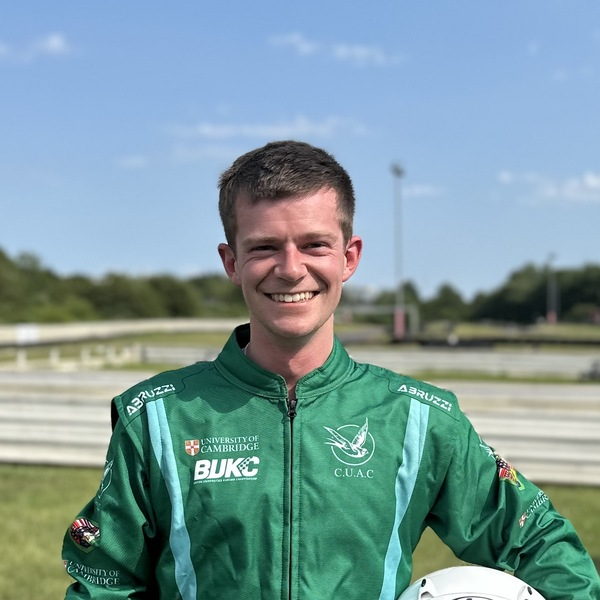
\includegraphics[height=0.09\textwidth]{images/adam_ormondroyd}

    }
\begin{columns}
    \column{0.5}

    \block{Clustering choice} {%
        \begin{minipage}{0.22\textwidth}
            \coloredbox{
                \centering
                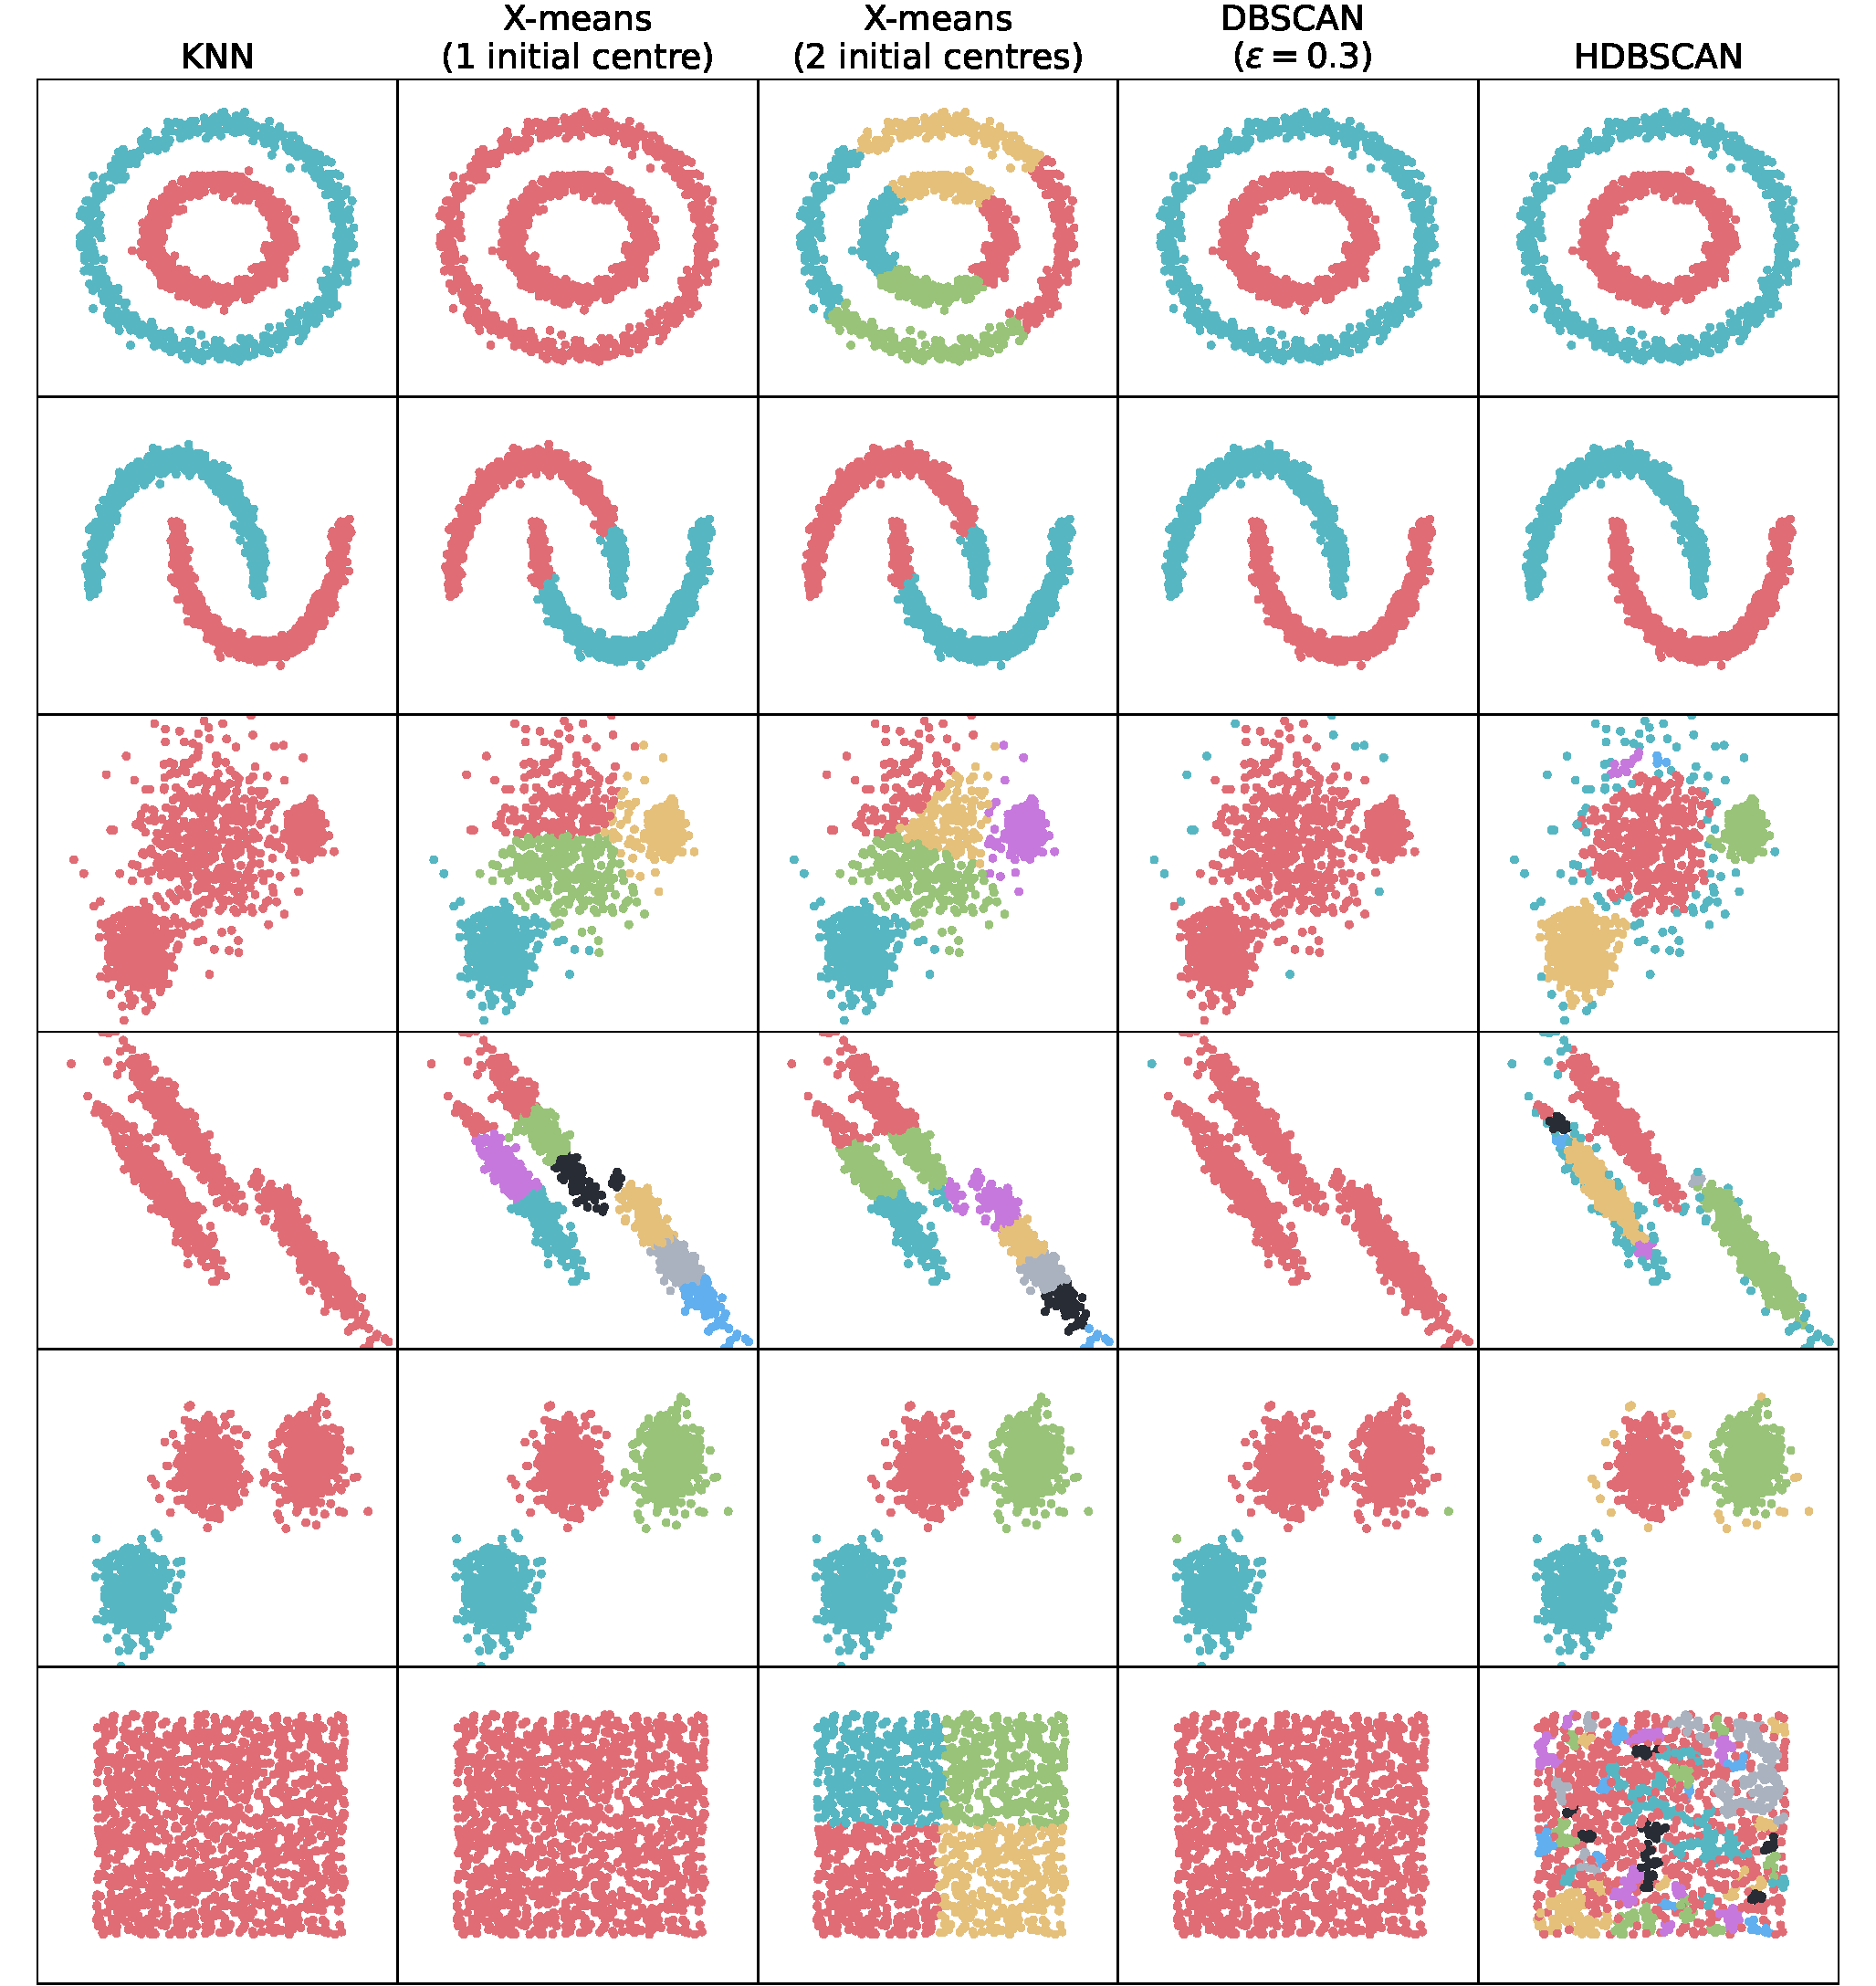
\includegraphics[width=0.9\textwidth]{images/clusterdam}

                2D demonstation of \polychord{} K-Nearest Neighbours, \texttt{pyclustering} X-means and \texttt{scikit-learn} (H)DBSCAN.
            }
        \end{minipage}
        \hfill
        \begin{minipage}{0.22\textwidth}
            The nested sampling algorithm \polychord{} was originally advertised suggesting that the user should experiment with their favourite cluster-identifying methods, but provides no guidance on how to do so \cite{polychorda, polychordb}. We have added an interface which allows the user to substitute any clustering strategy at the Python level, allowing for easier experimentation with alternatives such as the selection provided by \texttt{scikit-learn} and \texttt{pyclustering} \cite{sklearn, pyclustering}.

            Some algorithms are better suited than others to identifying posterior modes of nested sampling live points, for example K-means and spectral clustering need to be told the number of clusters to look for, others may not assign every point to a cluster. Some algorithms find clusters where there are none!
        \end{minipage}\\
   }
    \block{Application to cosmology $\mathcal P_\mathcal R(k)$}{%
        \begin{minipage}{0.28\textwidth}
            This investigation was initially motivated by a reconstruction of the primordial matter power spectrum $\mathcal P_\mathcal R(k)$ using flexknots \cite{flexknota, flexknotb}, and the Planck 2018 likelihoods \cite{planck2018v, planck2018viii}. Planck measured the $C_\ell$ multipole range $1\le\ell\le7000$, corresponding to $10^{-4}\le k/\si{\mega\parsec^{-1}}\le10^{-0.3}$ \cite{ppsr}. Flexknots are parameterisations of 1D functions, consisting of a series of splines (in this case linear) joined at knots. The number and positions of knots are determined by the data, which can be performed by either combining several runs with fixed number of knots, or the number of knots being itself a parameter. In the former case, we noticed that with three knots only the mode with the central knot towards the left was being fully explored.
        \end{minipage}
        \hfill
        \begin{minipage}{0.16\textwidth}
            \coloredbox{
                \centering
                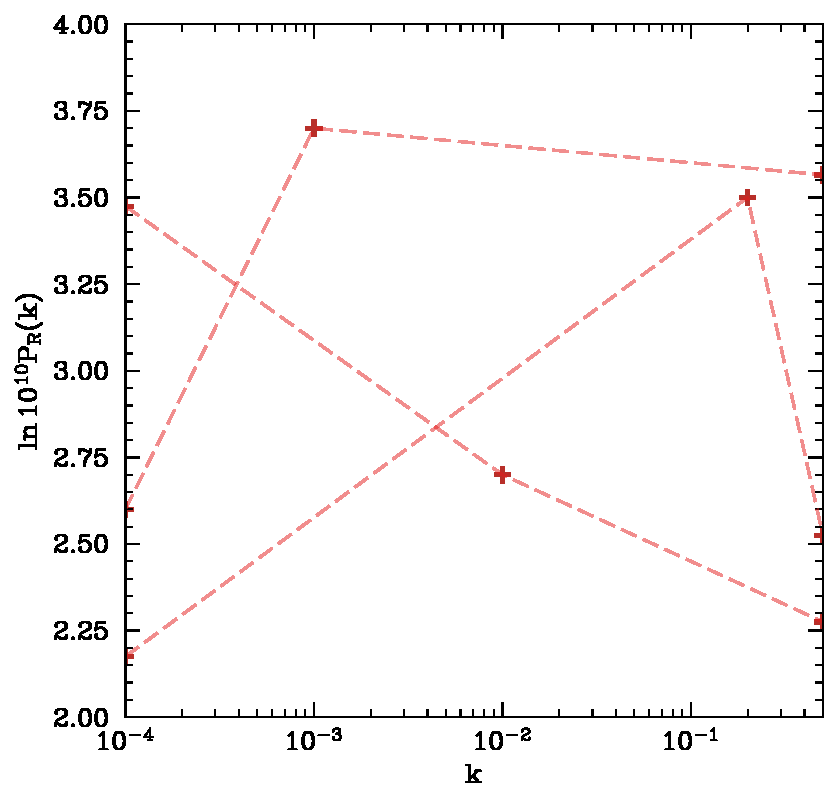
\includegraphics[width=0.9\textwidth]{images/amsterdam/example_flexknot}
                Examples of $\mathcal P_\mathcal R(k)$ flexknots with three knots each.
            }

            \coloredbox{
                \textbf{$\bf\mathcal L$-means}\centering\\

                algorithm here
            }
        \end{minipage}\\


        \polychord{}'s native K-nearest-neighbours clustering was unable to separate the positions of the central knot into two distinct clusters, so we explored both off-the-shelf clustering algorithms and approaches which include likelihood information. \\

        \begin{minipage}{0.22\textwidth}
            \innerblock{\rule[-0.6ex]{0pt}{2.5ex}K-nearest-neighbours}{
                \centering
                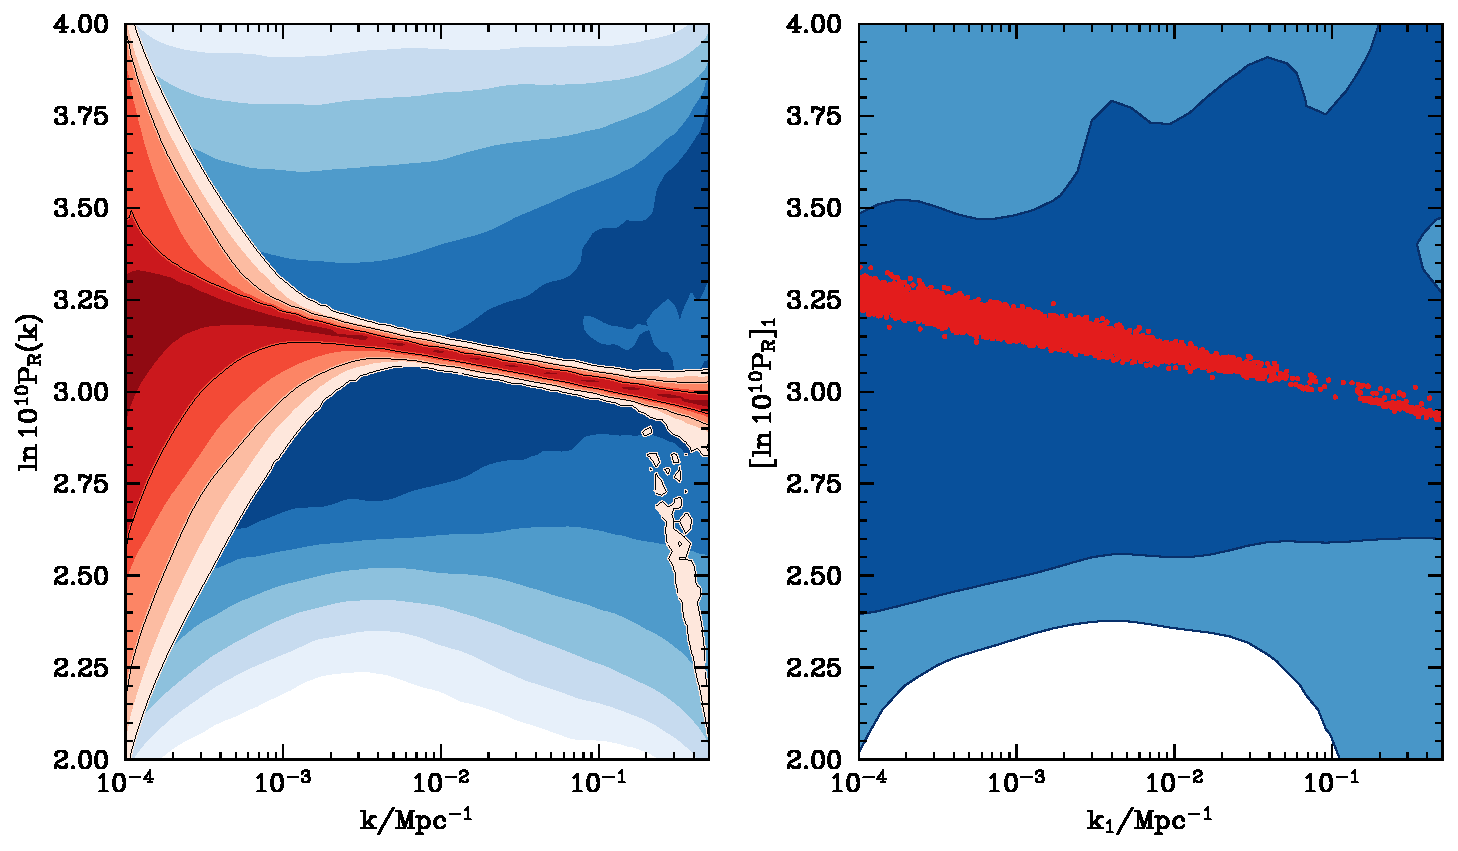
\includegraphics[width=0.9\textwidth]{images/amsterdam/knn}
            }
        \end{minipage}
        \hfill
        \begin{minipage}{0.22\textwidth}
            \innerblock{\rule[-0.6ex]{0pt}{2.5ex}X-means}{
                \centering
                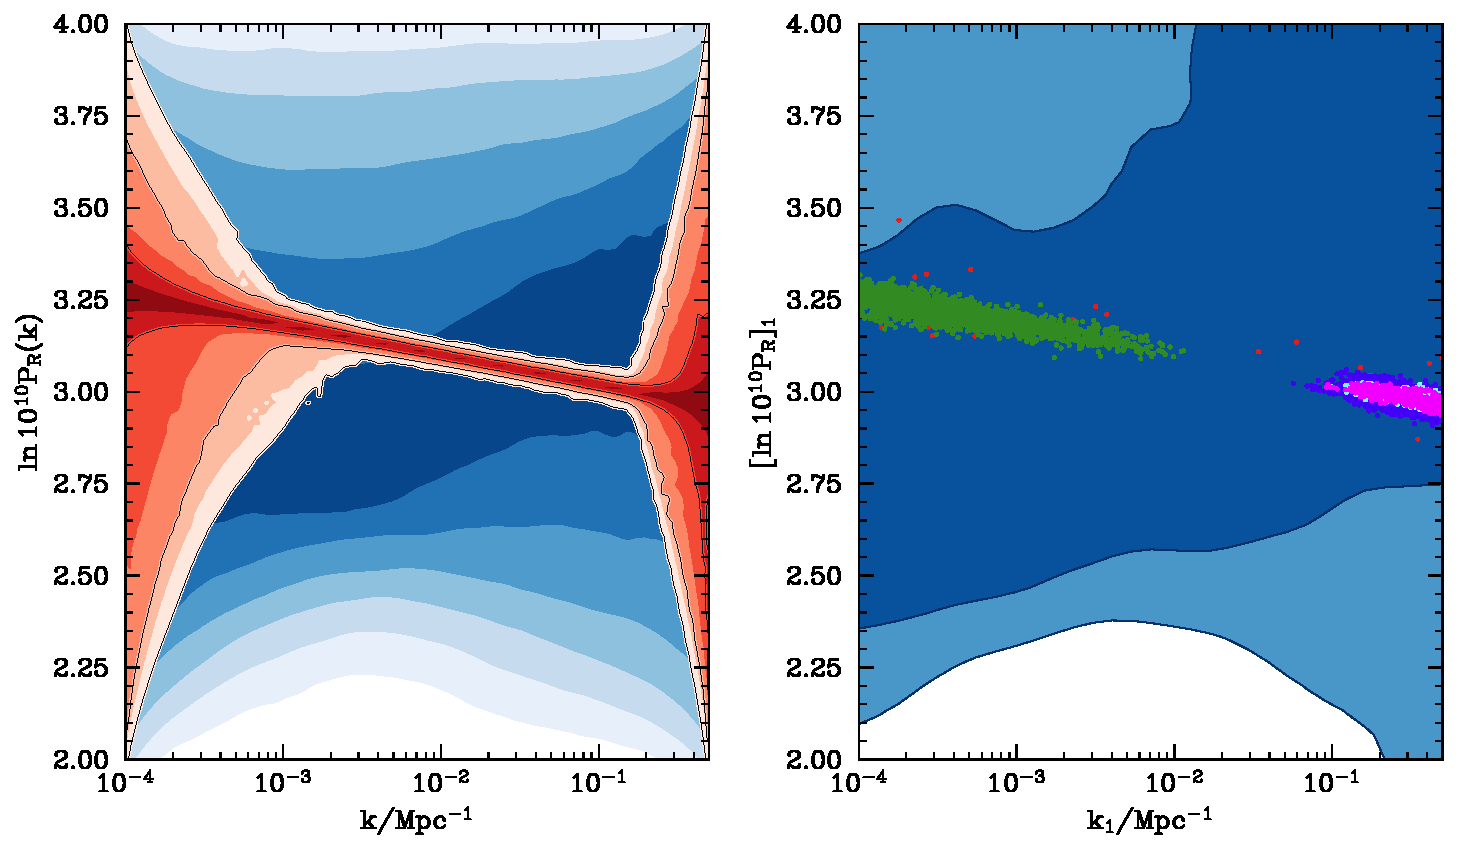
\includegraphics[width=0.9\textwidth]{images/amsterdam/xmeans}
            }
        \end{minipage}
        \begin{minipage}{0.22\textwidth}
            \innerblock{\rule[-0.6ex]{0pt}{2.5ex}DBSCAN}{
                \centering
                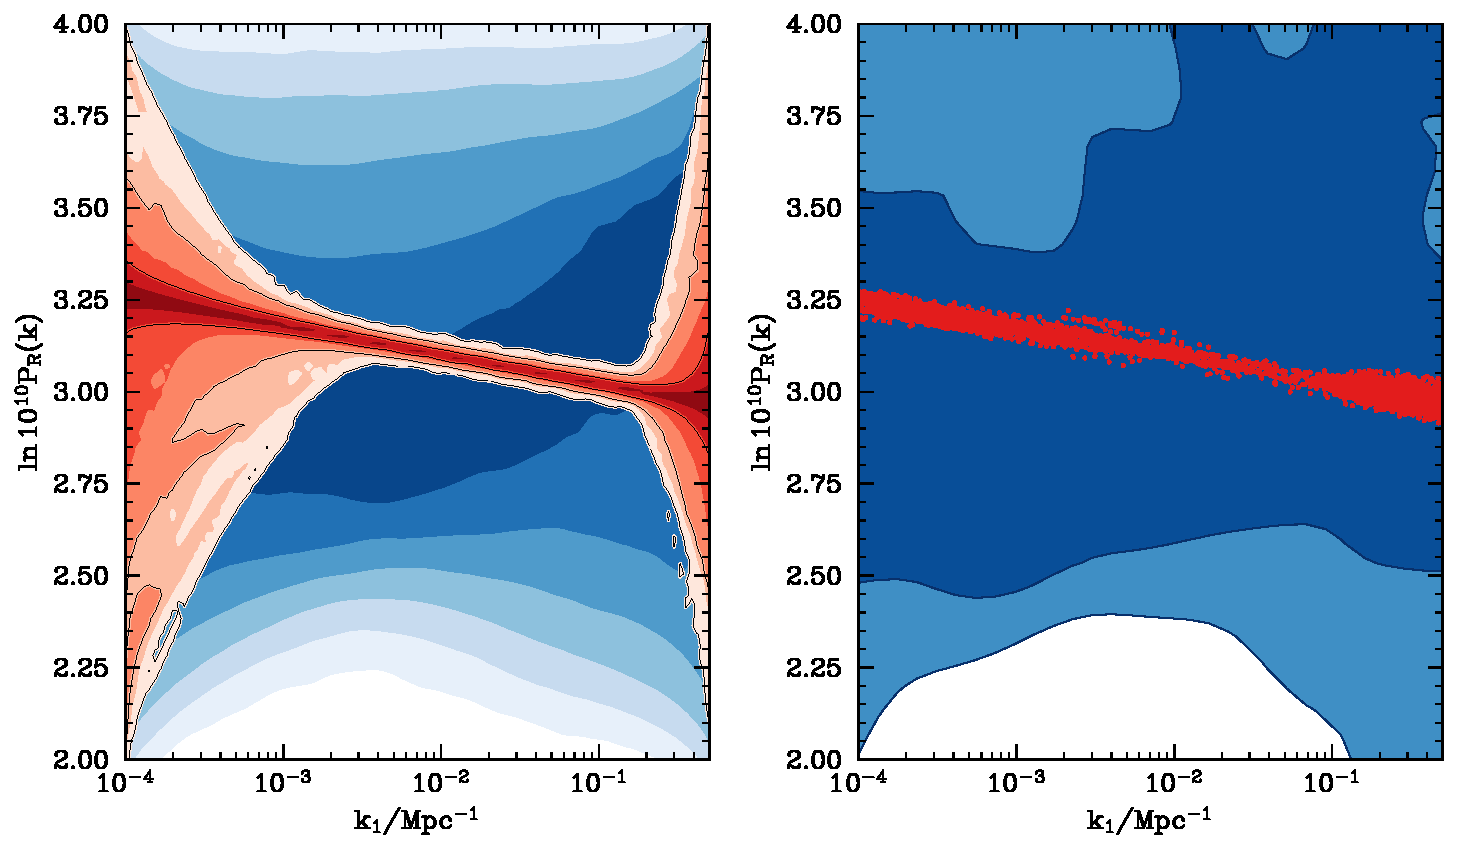
\includegraphics[width=0.9\textwidth]{images/amsterdam/dbscan}
            }
        \end{minipage}
        \hfill
        \begin{minipage}{0.22\textwidth}
            \innerblock{\rule[-0.6ex]{0pt}{2.5ex}using likelihood information}{
                \centering
                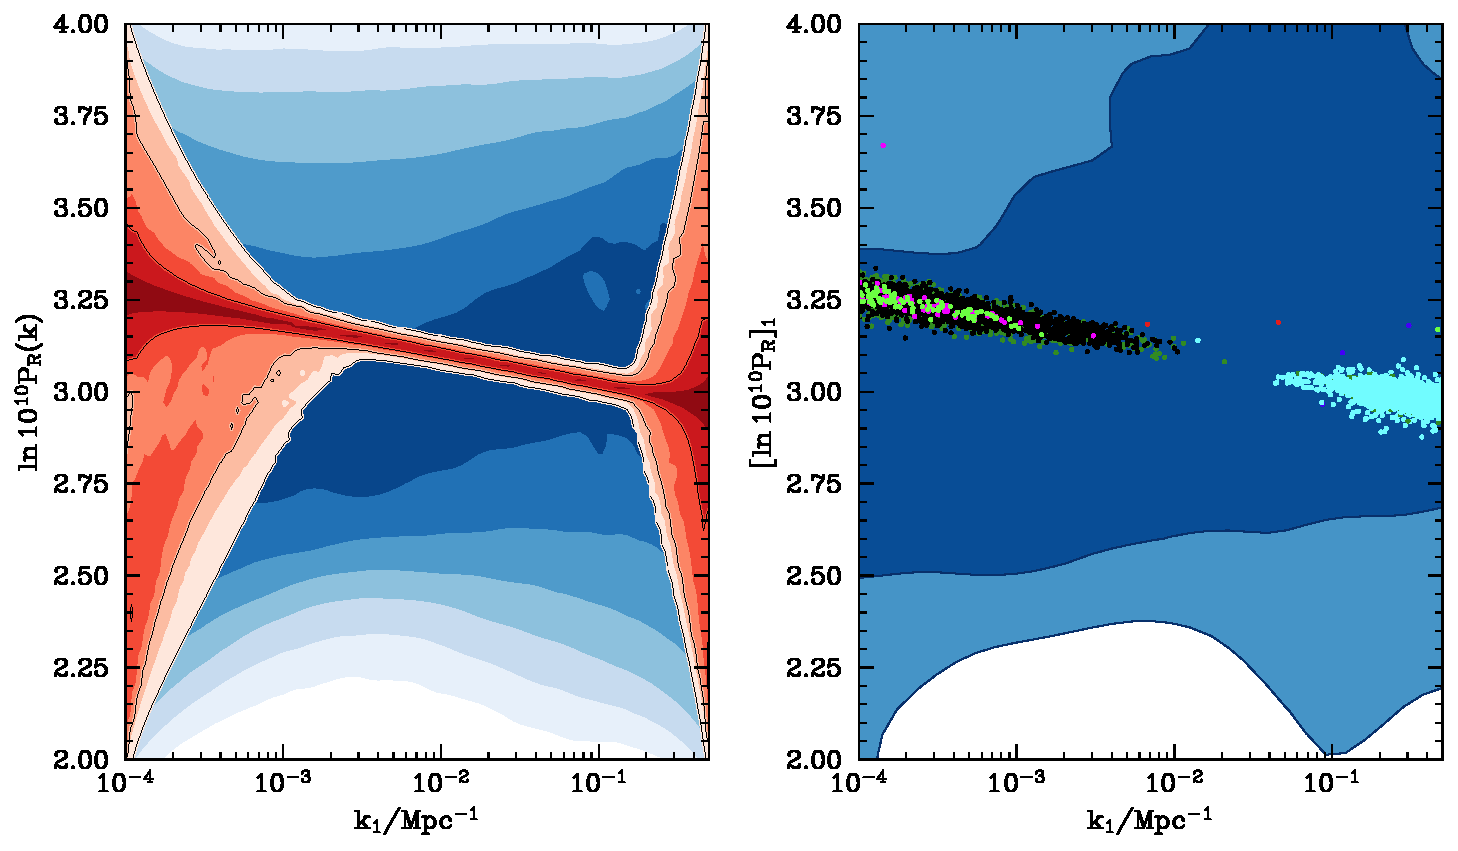
\includegraphics[width=0.9\textwidth]{images/amsterdam/convex}
            }
        \end{minipage}\\
        \coloredbox{K-nearest-neighbours and DBSCAN fail to separate the central knot into two clusters, while X-means does so reliably. The likelihood information approach was able to separate the central knot into multiple clusters, but also tended to over-cluster. Functional posterior plots created using \texttt{fgivenx} \cite{fgivenx}, and scatterplots showing clusters were created using a development branch of \texttt{anesthetic}\cite{anesthetic}.}
    }

    \column{0.5}

    \block{Classes of Nested Sampler}{
        Nested sampling algorithms have two main strategies for sampling new points from the prior:\\
        \begin{minipage}{0.22\textwidth}
            \innerblock{\rule[-0.6ex]{0pt}{2.5ex}Chain-based}{
                Taking a sufficiently long random walk within the likelihood contour from an existing live point will generate a new live point. For example, \polychord{} first uses the covariance matrix of the live points to whiten the space, then perform's Neal's slice sampling along orthogonal directions in that space \cite{polychorda, polychordb}. \texttt{dynesty} also implements both Neal's and Hamiltonian slice sampling, along with uniform sampling and random walks \cite{dynesty}.

                With multiple modes, contour whitening is ineffective, and a strategy is required to decide from which mode to sample since a random walk restricted by the likelihood contour will never reach another mode. \polychord{}, after identifying its clusters, picks one of the clusters at random in proportion to its prior volume.
            }
        \end{minipage}\hfill
        \begin{minipage}{0.22\textwidth}
            \innerblock{\rule[-0.6ex]{0pt}{2.5ex}Region-based}{
                Region-based samplers construct regions around the live points to approximate the likelihood contour, for example \texttt{MultiNest} constructs a series of ellipsoids \cite{multinesta, multinestb, multinestc}. These regions are usually expanded by some numerical factor to improve their chances of fully enclosing the likelihood contour, then a point is rejection-sampled from them. The curse of dimensionality means that these techniques are only effective up to $\mathcal O(10)$ dimensions, since the rejection sampling becomes too inefficient, or the expansion factor would have to be so low that significant regions of the likelihood contour would be missed. Multi-modality also causes inefficiency since the ellipsoids have to be very large to encompass all modes.
                \\
            }
        \end{minipage}\\
        \vspace{1em}

        \coloredbox{Hybrid methods combine the two approaches in an attempt to alleviate the dimensionality scaling of region-based methods, while reducing the number of likelihood evaluations made outside the contour \cite{nsmethods, dynesty, nestedfit, ultranest}.}

    }

    \block{Correlated cluster volumes}{%
        \begin{minipage}{0.22\textwidth}
            When a cluster $p$ is divided, the remaining prior volume $X_p$ is divided among its subclusters $X_i$. However, in nested sampling we do not have the precise prior volume, only its expectation value $\overline{X}$ and associated error. This is then divided according to the proportion of live points in each cluster $n_i$:
            \coloredbox{
            \begin{equation}
                \begin{aligned}
                \overline X_i &= \frac{n_i}{n_p} \overline X_p \text, \quad \overline{X_i^2} = \frac{n_i(n_i+1)}{n_p(n_p+1)} \overline{X_p^2} \text,\\
                \quad \overline{X_iX_j} &= \frac {n_i n_j}{n_p(n_p+1)} \overline{X_p^2} \text.
                \end{aligned}
                \nonumber
            \end{equation}
            }
        
        \end{minipage}\hfill
        \begin{minipage}{0.22\textwidth}
            \coloredbox{
            \centering
            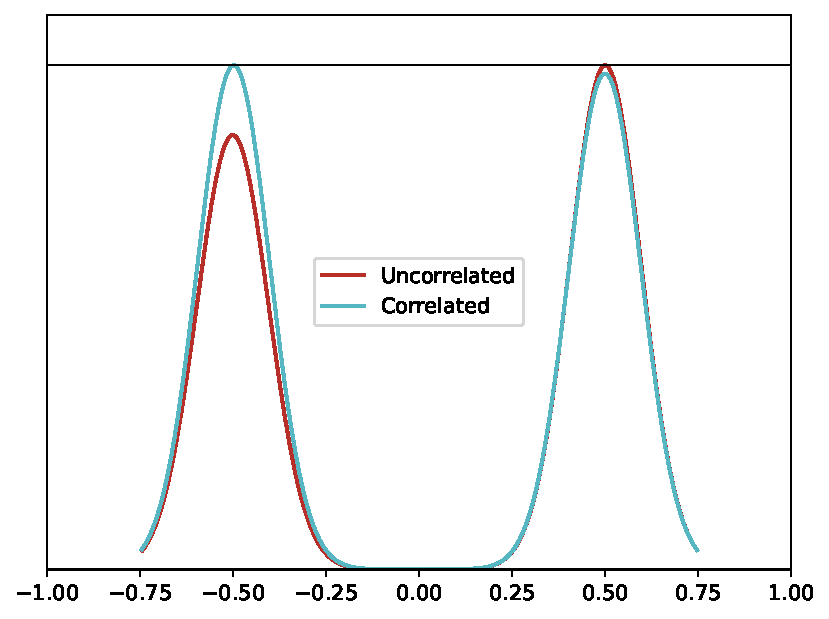
\includegraphics[width=0.9\textwidth]{images/volumes.pdf}

            KDE of posterior samples from twin 2D Gaussian likelihoods with 2000 live points, viewed along one of the axes.
            }
        \end{minipage}

        Since $\overline{X_iX_j} \neq \overline{X_i}\,\overline{X_j}$, the error on the prior volume of each cluster is correlated. This is important when deciding from which cluster to sample; currently \polychord{} chooses a cluster propotionally to its prior volume $\overline{X_i}$, but this neglects their correlation. We are experimenting with drawing a set of $X_i$ from their joint distribution before each live point is generated, which has improved posteriors of symmetric multi-modal likelihoods.\\

    }
    


    \renewcommand{\section}[2]{}%
    \block{References}{%
        \begin{minipage}[b]{0.35\textwidth}
            \bibliographystyle{unsrt}
            \tiny
            \bibliography{poster}
        \end{minipage}%
        
\includegraphics[width=0.1\textwidth]{images/QR.png}
    }

    \note[targetoffsetx=0.18\textwidth,targetoffsety=0.04\textwidth, connection,angle=135,radius=0.08\textwidth]{scan here for cool plots and gifs demonstrating clustering!}
\end{columns}
\end{document}
